\section{Packet Reception Rate}
\label{sec:packet_reception_rate}

The effect of temperature and other environmental factors on link quality has most thoroughly been investigated (\cite{Wennerstrom2013}, \cite{Boano2013}, \cite{Boano2014}, \cite{Zuniga2013}) with the conclusion that all measurements of link quality deteriorate with higher temperature, as one would expect.
However, Boano~\etal{} showed in their experiments that this behavior is not symmetrical, since heating the transmitter caused a more significant drop in \ac{PRR} than heating the receiver~\cite{Boano2013}.

To replicate these results we used the same experiment setup as described in Subsection~\ref{subsec:effects_of_temperature}, but with random payload as message content.
We fixed mote rotation to create a link that is just starting to deteriorate at $50\,^{\circ}\mathrm{C}$, so that at low temperatures the link is of good quality, while at very high temperatures the link will break.

In the experiment we increased the temperature of the mote in box 0 in steps of $5\,^{\circ}\mathrm{C}$ and $10\,^{\circ}\mathrm{C}$ up to $80\,^{\circ}\mathrm{C}$ and kept the mote on box 1 at constant $30\,^{\circ}\mathrm{C}$, while sending 180.000 messages back and forth.
Then we repeated this, but heated box 1 and kept box 0 temperature constant.
To cancel out environmental factors we ran this experiment four times over two days, so we could then pick the two results with the least interference.

For the evaluation we plotted the normalized \ac{PRR} of messages sent one mote and received by the other mote over temperature and time and included \ac{BER} and \ac{LQI} and \ac{RSSI} values to illustrate link quality.
Figure~\ref{fig:prr_link_01} shows messages sent from mote 0 addressed to mote 1 for both temperature cycles, while Figure~\ref{fig:prr_link_10} shows the opposite direction.
It becomes immediately clear that higher temperature of either transmitter or receiver makes the link worse, however, this behavior is neither linear nor symmetrical.

\subsection{Effects of temperature on \acs{PRR} and \acs{BER}}

In Figure~\ref{fig:prr_link_01} the decrease in \ac{PRR} is small and relatively symmetrical up to about $65\,^{\circ}\mathrm{C}$, however, past that point we see a dramatic change, with the increments in temperature translating very strongly into significant drops in \ac{PRR}.
The drop in \ac{PRR} is not symmetrical and becomes much more pronounced, when the receiver is heated than when the transmitter is heated, especially visible in the last increment from $70\,^{\circ}\mathrm{C}$ to $80\,^{\circ}\mathrm{C}$.

This asymmetry is even more extreme in link 1-0, shown in Figure~\ref{fig:prr_link_10}, where heating the receiver beyond $70\,^{\circ}\mathrm{C}$ will cause an almost complete loss of message reception.
Interesting is the little dip in \ac{PRR} around $50\,^{\circ}\mathrm{C}$ in Subfigure~\ref{fig:prr_link_10_receiver}, which was present in this link in all four experiments with varying intensity. We suspect that this is a non-linearity in the radio, cases of which have also been reported by Boano~\etal.

The \ac{BER} acts like an inverse function of \ac{PRR}, since higher \ac{BER} yields more messages with at least one bit error.
Noise on \ac{PRR} is visible in the standard deviation of \ac{BER} as exemplified by Subfigure~\ref{fig:prr_link_10_transmitter}.

\subsection{Effects of temperature on \acs{LQI} and \acs{RSSI}}

The \ac{LQI} is a very good mirror of the \ac{PRR} of messages without error.
When the receiver is kept at a constant temperature, the values decrease almost linearly with temperature of the transmitter.
This is not the case when the receiver is heated, where a linear correlation to temperature does not to exist, but is still very similar to the behavior of \ac{PRR}.
We therefore can confirm, that \ac{LQI} is a good source for an estimate on \ac{PRR}.

This is very much not the case with \ac{RSSI}, which has much lower resolution that \ac{LQI} and exhibits hysteresis and non-linearities~\cite{Boano2013}.
While in Figure~\ref{fig:prr_link_01}, \ac{RSSI} ends up being lower when the receiver is heated than when it is constant, Figure~\ref{fig:prr_link_10} shows very similar values, even though \ac{PRR} is radically different.

It is also noteworthy that contrary to \ac{LQI}, \ac{RSSI} attempts to describe signal strength (\ie the power level being received by the antenna), which of course does not change, when the transmitter is at constant temperature.
Therefore, without temperature information, the \ac{RSSI} value is misleading, since it represents the power level not at the antenna, but at the signal amplifying stage 
Therefore \ac{RSSI} is usable for a very inaccurate estimate of link quality at best, with little to no difference between receiver and transmitter temperature.

\begin{figure}[t]
	\subfigure[Constant receiver, increasing \newline transmitter temperature.] {
		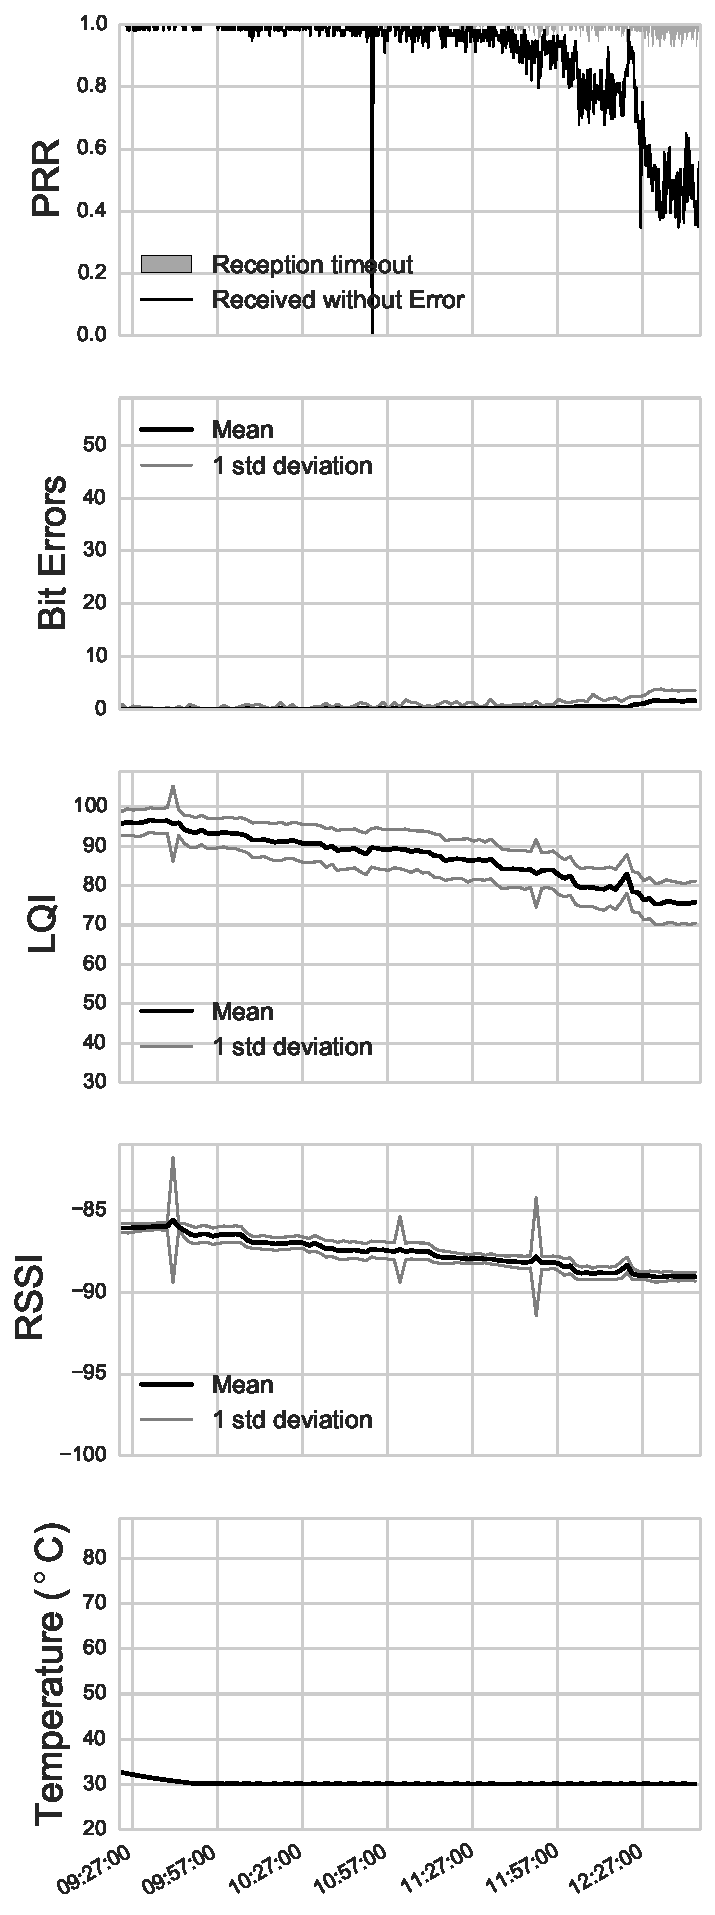
\includegraphics[width=0.475\columnwidth]{figures/prr_0-1_transmitter}
		\label{fig:prr_link_01_transmitter}
	}
	\subfigure[Increasing receiver, constant \newline transmitter temperature.] {
		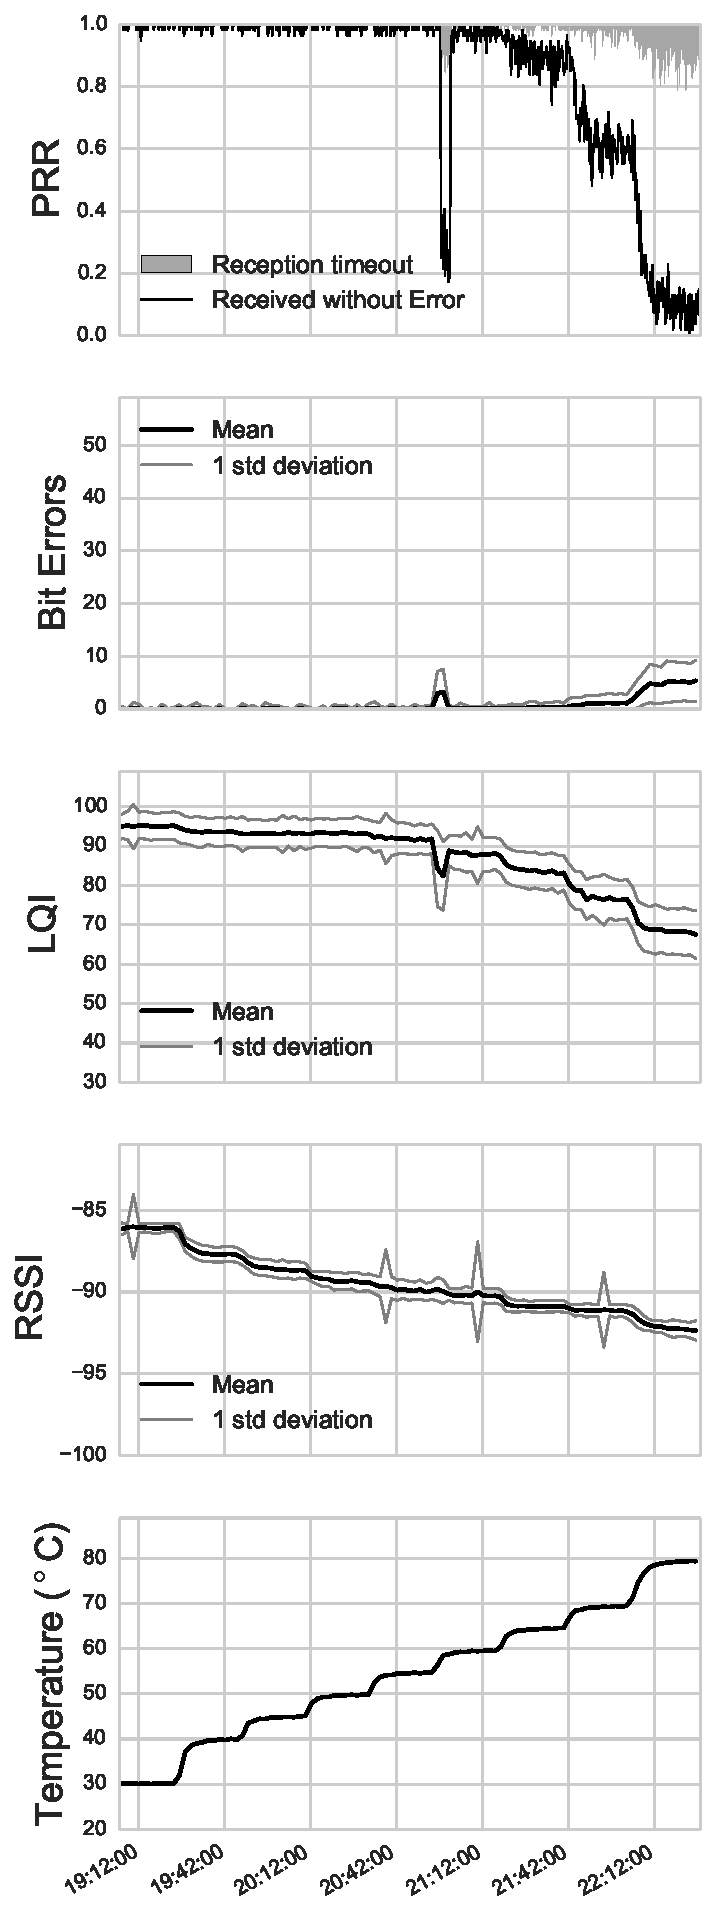
\includegraphics[width=0.475\columnwidth]{figures/prr_0-1_receiver}
		\label{fig:prr_link_01_receiver}
	}
	\caption{\acs{PRR} and link quality of messages received by mote \textbf{1} vs. temperature. For transmitter temperature see Figure~\ref{fig:prr_link_10}.}
	\label{fig:prr_link_01}
\end{figure}

\begin{figure}[t]
	\subfigure[Increasing receiver, constant \newline transmitter temperature.] {
		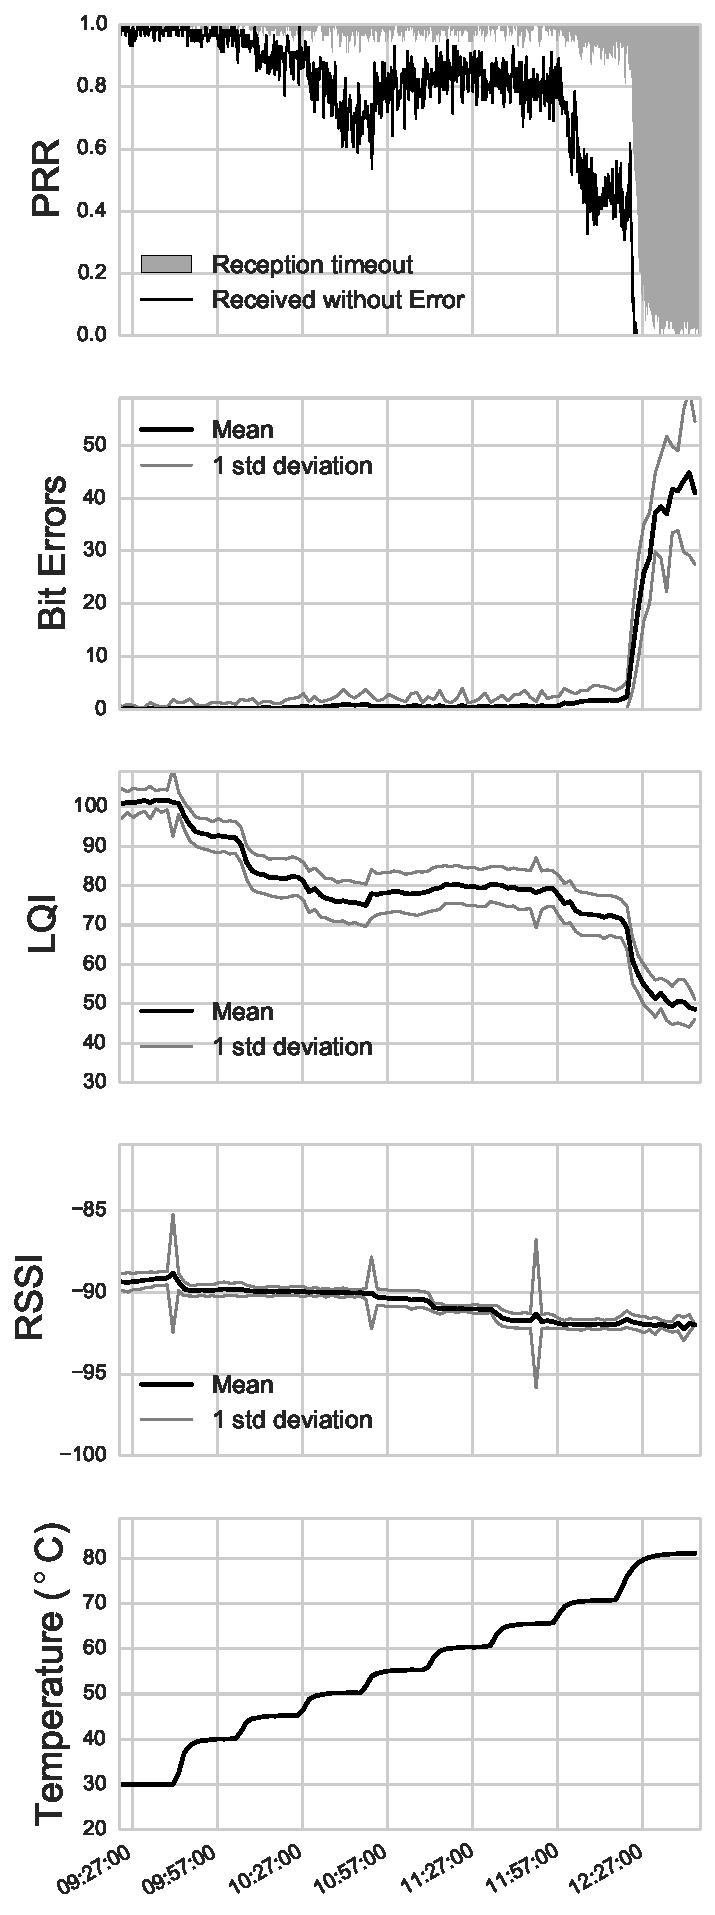
\includegraphics[width=0.475\columnwidth]{figures/prr_1-0_receiver}
		\label{fig:prr_link_10_receiver}
	}
	\subfigure[Constant receiver, increasing \newline transmitter temperature.] {
		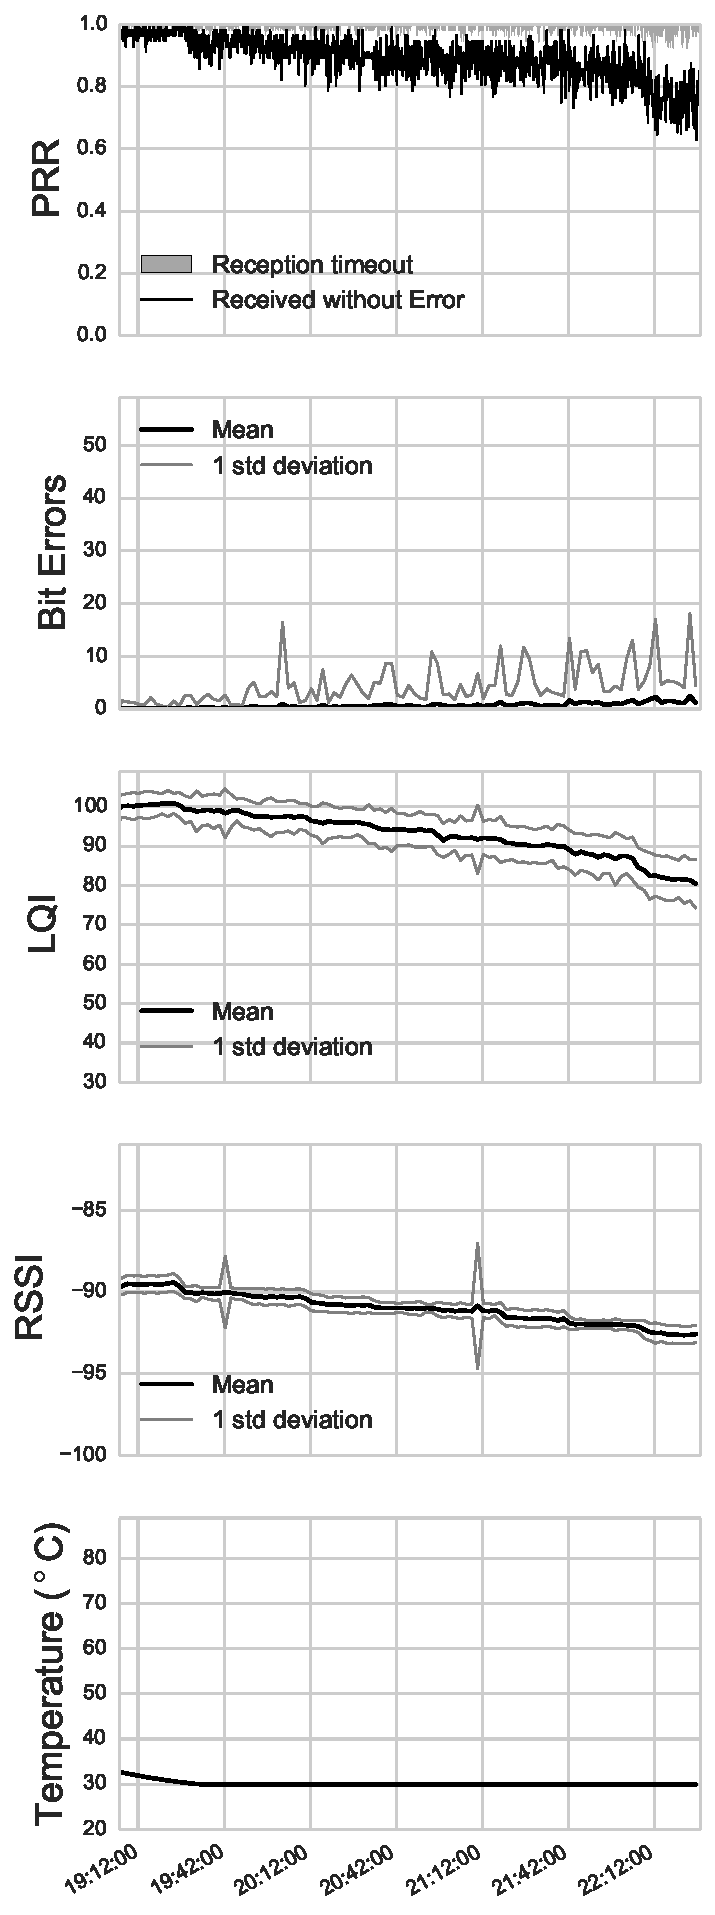
\includegraphics[width=0.475\columnwidth]{figures/prr_1-0_transmitter}
		\label{fig:prr_link_10_transmitter}
	}
	\caption{\acs{PRR} and link quality of messages received by mote \textbf{0} vs. temperature.  For transmitter temperature see Figure~\ref{fig:prr_link_01}. The asymmetry in \acs{PRR} shows much more cleary here.}
	\label{fig:prr_link_10}
\end{figure}

\subsection{Discussion}

These results are not necessarily incompatible with the findings of Boano~\etal{}, since the authors only looked at an effective temperature range of $0 - 65\,^{\circ}\mathrm{C}$, which is exactly the range, where we see little asymmetry in our experiment.
It is therefore feasible that there are link configurations in this temperature range, where this behavior can manifest itself.
However, our data strongly implicates the receiver as being more vulnerable than the transmitter to an increase in temperature, especially above $65\,^{\circ}\mathrm{C}$.

This link asymmetry can lead to some interesting situations, where a mote at high temperature is able to transmit messages, but not receive them.
Looking at their own temperature, mote would receive another hint in whether the lack of received messages is caused by a missing transmitter, or by its own disability to receive messages.
For example, when no messages are received after a timeout, a failure of the transmitter is more likely when the receiver is at low temperature than at high temperatures.

In a system that makes smart decisions based on information from multiple motes, such information could be used to judge whether the system is still functionally intact and then trigger a backup program, which reacts autonomously to the local sensor data collected but still notifies the rest of the network of its actions.
Motes that are not in this backup mode can very likely receive these transmissions and augment the group decisions with the constraints of these autonomously acting motes.
Therefore a failure of the entire system is delayed or prevented, by using controlled degradation of the system, which might not be as smart as before, but at least still providing a rudimentary service.
































